\Lecture{Jayalal Sarma}{Oct 19, 2020}{18}{Introduction to Ramsey Numbers}{Shivlal Gangesh}{$\alpha$}{JS}
\section{Introduction}
Till now we have seen advanced versions of the discrete mathematics topics we already know. Now we are going to get into Extremal combinatorics. Here we are interested in questions of the form 
\begin{itemize}
\item \textit{If this structure appears, then what is the minimum/maximum size of the object?}
\item \textit{If the size is at least this much , then what kind of structures appear in the object?}
\item \textit{What is the minimum size of the collection such that it is guaranteed to have certain property?}
\end{itemize}
In general we are interested in the extreme behaviors in combinatorics. The classic example we start with is an extension to an example that we have done in the beginning of the course as an Application of Pigeon Hole Principle.
\section{Starting Point} \label{R(3,3)}
\begin{theorem}
Six people meet in a party. Then either there exist three people who are friends with each other or there exist three people who are strangers with each other.(Note : Any two people can either be friends or strangers)
\end{theorem}
We are interested in proving the above statement. Lets look into two different approaches
\subsection{Model 1 (Using Cliques and Independent Sets)}
\begin{description}
   \item[Model] Let us represent the problem as a $6$ vertex graph $G(V,E) $with each person corresponding to a vertex. $(u,v) \in E$ if and only if person $u$ is a friend of person $v$.
In this Model the original statement can be reformulated as
\item[Statement]
\textit{Any graph on $6$ vertices must either have a clique on $3$ vertices or an independent set on $3$ vertices.
\item}
\begin{proof}
 Consider any vertex $v$ in the graph G, without loss of generality we can assume that the degree of $v$ is greater than or equal to $3$  because suppose it is not the case then consider $\overline{G}$ ; as $\textrm{Cliques in }G \leftrightarrow \textrm{Independent Sets in } \overline{G} $.\\
 Let the $3$ neighbours of $v$ be $a$, $b$ and $c$. Consider the two exhaustive cases :
 \begin{description}
    \item[Case 1 : There are no edges among $a$, $b$ and $c$]
    $ $ \newline
    Here we have $\{a, b, c\}$ as the 3-Independent Set
    \item[Case 2 : There is at least one edge among $a$, $b$ and $c$ ]
    $ $ \newline
    Let $(a,b) \in E$ be that edge, then we have $\{v, a, b\}$ as the 3-clique
 \end{description}
Therefore the given statement holds true.
\end{proof}
\item[Proof for tightness]
To prove that this is tight we need to show there is a graph with $5$ vertices such that it does not have 3-clique and 3-Independent Set. Given below is one such  example
\begin{figure}[h!]
    \centering
    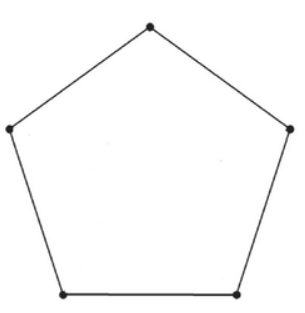
\includegraphics[width=0.2\linewidth]{images/r33counter_example.png}
    \caption{5-vertex graph with no 3-clique and no 3-Independent Set}
\end{figure}
\end{description}
\subsection{Model 2 (Using Graph Edge colouring)}
\begin{description}
   \item[Model]
   Let us represent the problem as 2-edge coloring of a $K_6$ graph with each vertex corresponding to a person. Color the edge $(u,v)$ with \textit{red} if $u$ and $v$ are friends, color it with \textit{blue} if $u$ and $v$ are strangers.
In this Model the original statement can be reformulated as
\item[Statement]
\textit{For any 2-edge colouring of $K_6$, there must exist either  a red $K_3$  or a blue $K_3$ }
\item
\begin{proof}
 Consider any Red,Blue-edge coloring of $K_6$. Consider any vertex $v$, the degree of $v$ is $5$ as the graph is a complete graph. By Pigeon Hole Principle , $v$ must have either $3$ red edges incident on it or $3$ blue edges incident on it. Consider the case when $v$ is incident on with $3$ red edges. Let the 3 neighbours of $v$ be $a$, $b$ and $c$.  Now there are 2 cases :
 \begin{description}
    \item[Case 1 : There is no red colored edge among $(a,b)$, $(b,c)$ and $(c,a)$ ]
    $ $ \newline
    Then all the three edges $(a,b)$, $(b,c)$ and $(c,a)$ are colored blue. Therefore $\{a, b, c\}$ forms a blue $K_3$
    \item[Case 2 : There is at least one red colored edge among $(a,b)$, $(b,c)$ and $(c,a)$ ]
    $ $ \newline
    Let $(a,b)$ be the red colored edge, then $\{v, a, b\}$ forms a red $K_3$
 \end{description}
 Therefore the given statement holds true.
\end{proof}
\item[Proof for tightness]
To prove that this is tight we need to show there is a 2-edge coloring of $K_5$ Such that it does not have red $K_3$ and blue $K_3$. Given below is one such  example
\begin{figure}[h!]
    \centering
    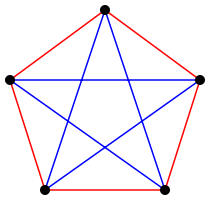
\includegraphics[width=0.2\linewidth]{images/k5counter_example.png}
    \caption{2-edge coloring of $K_5$ with no red $K_3$ and no blue $K_3$}
\end{figure}
\end{description}

Generalizing the above problem with arbitrary red $k_p$ and blue $k_q$ has been extensively studied by Ramsey and has led to the definition of Ramsey numbers.
\section{Ramsey numbers}
\begin{definition}[Ramsey number]
The Ramsey number denoted by $R(p,q)$ is the minimum number of vertices say $n$ such that any 2-edge coloring of $K_n$ must have either a red $K_p$ or a blue $K_q$.\\
(\textbf{Or equivalently as})\\
The minimum number of vertices ($n$) such that any graph on $n$ vertices must either have a clique on $p$ vertices or an independent set on $q$ vertices.
\end{definition}

\subsection{Some Observations}
\begin{property}
$R(3,3)=6$
\end{property}
This is the direct formulation of the example we have done previously in \ref{R(3,3)}
\begin{property}
$R(p,q) = R(q,p)$
\end{property}
The colors \textit{red} and \textit{blue} are just placeholders for two colors, thus swapping the colors will still preserve the Ramsey number property. Therefore $R(p,q) = R(q,p)$.
\begin{property}
$\forall l \geq 1 \quad R(l,1) = 1$
\end{property}
The existence of a blue $K_1$ is nothing but the presence of single vertex and any graph with a single vertex satisfies this property. Therefore $R(l,1) = 1$


\section{Existence of R(p,q)}
The Proof for the existence of $R(p,q)$ is due to Erdős–Szekeres. The existence was proved by providing an upper bound as a recurrence relation as follows :
\begin{theorem}
$$\forall p,q \geq 2 \quad R(p,q) \; \leq \; R(p,q-1) + R(p-1,q) $$
\end{theorem}
\begin{proof}
 Let us prove this by mathematical induction on $n$ where $n=p+q$.
 \begin{description}
    \item[Idea] To show the upper bound for $R(p,q) \leq n$ , we must argue that for any 2-edge coloring of $K_n$ there exist a red $K_p$ or blue $K_q$

   \item[Base case] $p=q=2$
$$R(2,2) \leq  R(2,1) + R(1,2)  $$
$$2 \leq 1+1$$
Hence it holds true for the base case.
   \item[Induction Hypothesis]
Assume the recurrence relation is true for $n<l$. Then we need to prove it for $n=l$. Let $n=R(p-1,q)+R(p,q-1)$. Let $w$ be any vertex in $G$ ($K_n$) and consider any $2$ -edge coloring of $G$. Let $H_1$ be the subgraph of $G$ formed from the vertices sharing a red-edge with $v$ and $H_2$ be the the subgraph of $G$ formed from the vertices sharing a blue-edge with $v$.
\begin{description}
   \item[Case 1 : There are at least $R(p-1,q)$ many red edges incident on vertex $w$]
   $ $ \newline
   $H_1$ is a complete graph on $R(p-1,q)$ vertices with 2-edge coloring. By definition and Induction Hypothesis we have that there exist a red $K_{p-1}$ or blue $K_q$ in $H_1$. So in graph $G$ (along with vertex $w$) there exist a red $K_p$ or blue $K_q$
   \item[Case 2 : There are at least $R(p,q-1)$ blue edges incident on vertex $w$]
      $ $ \newline
      $H_2$ is a complete graph on $R(p,q-1)$ vertices with 2-edge coloring. By definition and Induction Hypothesis we have that there exist a red $K_p$ or blue  $K_{q-1}$ in $H_2$. So in graph $G$ (along with vertex $w$) there exist a red $K_p$ or blue $K_q$.
\end{description}
   \end{description}
   
\end{proof} 
   
\Lecture{Jayalal Sarma}{Oct 21, 2020}{19}{Computing Ramsey Numbers and Multidimensional Ramsey numbers}{Shivlal Gangesh \& Reetwik Das}{$\alpha$}{JS}
\section{Generalizing Ramsey numbers}
\begin{definition}[3-dimensional Ramsey numbers]
$R_3(p,q,r)$ is the minimum number $n$, such that any 3-edge coloring $K_n$ must have either a red $K_p$ or a blue $K_q$ or a green $K_r$
\end{definition}
\begin{definition}[$k$-dimensional Ramsey numbers]
$R_k(s_1,s_2,\cdots ,s_k)$ is the minimum number of vertices $n$ such that for any $k$-edge coloring of $K_n$  there must exist an $i$ such that there is a $K_{s_i}$ of colour $i$
\end{definition}

\section{Some Observations}
\begin{property}
$R(2,p)=p$
\end{property}
\begin{proof}
$ $ 
 \begin{description}
    \item[Case1 : $R(2,p) \leq p$]
    $ $ \newline
    Any 2-coloring of $K_p$ must have either a red $K_2$ or blue $K_p$. This is true because either there can exist a red edge (red $K_2$) or no red edge (blue $K_p$) in $K_p$
    \item[Case 2 : $R(2,p) \geq p$]
    $ $ \newline
    There exist a 2-coloring of edges of $K_{p-1}$ such that no red $K_2$ exists and no blue $K_p$ exists. Coloring all the edges of $K_{p-1}$ with blue will result in no red $K_2$ and no blue $K_p$ in $K_{p-1}$
 \end{description}
\end{proof}
\begin{claim}
$$ R(p,q) \leq {p+q-2 \choose p-1} $$
\end{claim}
\begin{proof}
 \begin{align*}
     R(p,q) &\leq  R(p,q-1) + R(p-1,q) && \textrm{(Erdos-Szekeres recurrence relation)} \\
     &\leq {p+(q-1)-2 \choose p-1} + {p-1+q-2 \choose p-2} \\
     &\leq {p+q-3 \choose p-1} + {p+q-3 \choose p-2} \\
     &\leq {p+q-2 \choose p-1}  && ({n+1 \choose k+1} = {n \choose k+1} +{n \choose k})
 \end{align*}

\end{proof}
\section{Explicit Computation of R(3,4)}
We don't know the exact values of Ramsey numbers for higher values as their computation becomes very hard. There is this famous saying by Paul Erdos on the difficulty of computing Ramsey numbers that
\begin{description}
   \item[Paul Erdos on Ramsey numbers] 
   $ $ \newline
\textit{   "Suppose aliens invade the earth and threaten to obliterate it in a year's time unless human beings can find the Ramsey number for red five and blue five. We could marshal the world's best minds and fastest computers, and within a year we could probably calculate the value. If the aliens demanded the Ramsey number for red six and blue six, however, we would have no choice but to launch a preemptive attack."}
\end{description}
 So let us now try to calculate the value of $R(3,4)$. 
 \begin{claim}
 $$ R(3,4) = 9 $$
 \end{claim}
 \begin{proof}
 $ $
 Consider any 2-coloring of $K_9$ and call it as $G$. We need to prove that $G$ has either a red $K_3$ or a blue $K_4$. Any vertex in $G$ can have it's incident edges as one of the three cases below
  \begin{itemize}
  \item \textbf{Case 1 : }There are at least $4$ red edges going out of the vertex
  \item \textbf{Case 2 : }There are at least $6$ blue edges going out of the vertex
  \item \textbf{Case 3 : }There are exactly $3$ red edges and $5$ blue edges going out of the vertex
  \end{itemize}
 However note that not all vertices in $G$ come under \textbf{Case 3} because, if so then the total sum of degrees of all vertices becomes odd which is not possible. So let $v$ be a vertex in $G$ which does not fall under \textbf{Case 3}. Then
 \begin{description}
    \item[Case 1 : There are at least 4 red edges going out of $v$ ]
    $ $ \newline
    Let $H_1$ be the subgraph of $G$ formed from the four vertices which are sharing the red edge with $v$.  Since we know that $R(2,4)=4$, $H_1$ with 4 vertices must have a red $K_2$ or a blue $K4$, So along with vertex $v$, $G$ must have a red $K_3$ or a blue $K_4$.
    \item[Case 2 :There are at least 6 blue edges going out of $v$]
    $ $ \newline
    Let $H_2$ be the subgraph of $G$ formed from the six vertices which are sharing the blue edge with $v$. Since we know that $R(3,3)=6$, $H_2$ with 6 vertices must have a red $K_3$ or a blue $K3$, So along with vertex $v$, $G$ must have a red $K_3$ or a blue $K_4$.
    \item[Proof for tightness]
    $ $ \newline
    To prove that $9$ is tight, we need to show that there is a 2-coloring of $K_8$ such that it does not have red $K_3$ or blue $K_4$. Given below is one such  example
\begin{figure}[h!]
    \centering
    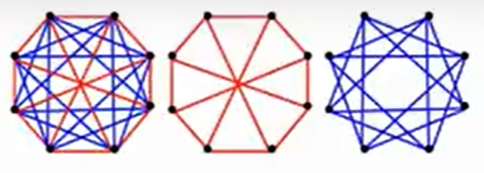
\includegraphics[width=0.5\linewidth]{images/R34counter_example.png}
    \caption{2-coloring of $K_8$ with no red $K_3$ and no blue $K_4$}
\end{figure}
 \end{description}
  
 \end{proof}
 As the values $p$, $q$ increases we can only calculate the range of the Ramsey number. The following is a table with value or range of Ramsey numbers for the first few natural numbers.
 \begin{figure}[h!]
    \centering
    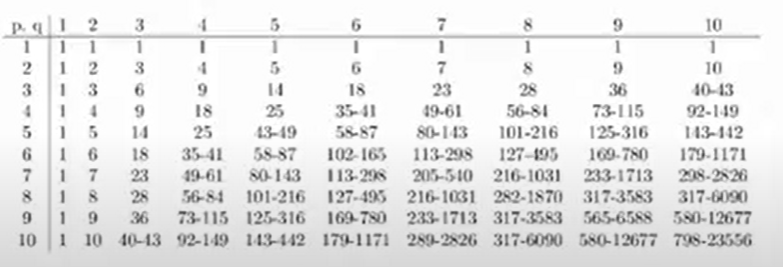
\includegraphics[width=1\linewidth]{images/RamseyTable.png}
    \caption{Table for $R(p,q)$}
\end{figure}

% Reetwik Started from here

\section{Multidimentional Ramsey numbers}
\begin{definition}
$R_k(S_1,S_2,..S_k)$ is mininum number $n$ such that any $k$-edge coloring of $K_n$ must have $K_{S_i}$ of color $i$ for some $i \in \{1,2..k\}$
\end{definition}
We need to show that why should exist $R_k(S_1,S_2,..S_k)$.
\begin{claim}
$$R_k(S_1,S_2,..S_k) \leq R_{k/2}(R(S_1,S_2), R(S_3,S_4).... R(S_{k-1},S_k))$$
\end{claim}
\begin{proof}
Let $n =  R_{k/2}(R(S_1,S_2), R(S_3,S_4).... R(S_{k-1},S_k))$\\
Consider $K_n$ and any K-edge coloring of the edges of $K_n$\\

We need to show that $\exists S_1$ clique of color 1 or $S_2$ clique of color 2.\\
Consider colors paired up and rename them $\{1,2\} = 1, \{3,4\} = 2, ... \{k-1,k\} = k/2$ \\
By the definition of $R_{k/2}$ we are guaranteed $\exists i$ such that $\exists$ a clique of size $R(S_{2i-1},S_{2i})$ of color $i$.\\

After we uninterpret the color $i$ as the original pair of colors we get a 2-coloring of the clique that we have $R(S_{2i-1},S_{2i})$\\
By the definition of $R_2$ we know that $\exists$ a $S_{2i-1}$ clique of color $2i-1$ or $S_{2i}$ clique of color $2i$.
\end{proof}

\section{Fermat's last theorem}
We know from Pythagoras theorem that $x^2 +y^2 = z^2$ has integral solutions. But we want to know if this equation has any integral solutions for any power greater than $2$.
\begin{theorem}
$x^n +y^n = z^n$ doesn't have any integral solutions $\forall n>2$.
\end{theorem}

\Lecture{Jayalal Sarma}{Oct 22, 2020}{20}{Finite fields}{Reetwik Das}{$\alpha$}{JS}

\subsection{Finite fields}
$x^n +y^n = z^n$ does have integeral solutions for finite fields such as for $Z_p$.\\
$Z_p = \{0,1,....p-1\}$ and addition and multiplication are $modulo$ $p$ within this field.\\

\begin{definition}
$Z_p^*$ is a cyclic group $\{1,2,3....p-1\}$
\end{definition}

\begin{claim}
If $p$ is a prime then $Z_p^*$ is generated by a single element, and the element is known as the generator.
\end{claim}

Fermat's last theorem is completely algebraic to connect it to coloring we need a tool.
\begin{theorem}
\textbf{Schur's theorem :} If $r \geq 0$ positive integer then. $\exists$ integer $S(r)$ such that if we color $\{1,2,....S(r)\}$ vertices with $r$ colors then $\exists x,y,z$ in the set and $x+y =z$
\end{theorem}
\begin{proof}
Given an $r$, Let $S(r) = R_r(3,3,3,...3)$\\
Consider $K_n$, $n = S(r)$ by the definition if we color the edges of $K_n$ using $r$ colors then we are guaranteed a monochromatic $K_3$.\\
We are given a coloring $\{1,2,...S(r)\}$\\
Define a coloring for edges in $K_n$.\\
Associate vertices of $K_n$ with elements in $\{1,2,...S(r)\}$ \\
$\forall a,b\in V$ the color of edge $(a,b) $ = color of $|a-b|$\\

Let $\{\alpha, \beta,\gamma\}$ be the vertices of the monochromatic triangle.
Let $x = \alpha - \beta$, $y = \beta - \gamma$ and $z = \alpha - \gamma$ then $x,y,z$ have the same color.
It also satifies the equation $x+y =z$.
 
\end{proof}

\begin{theorem}
$\forall m \exists q$ such that $\forall p\geq q$ in $Z_p$ ($p$ is a prime) \\
$x^m +y^m = z^m$ has a solution.
\end{theorem}
\begin{proof}
Given $m$ from $ x^m +y^m = z^m$\\
$p=q=S(m)+1$ by Schur's theorem any coloring of $\{1,2...q\}$ must have a triplet $a+b = c$.\\
$Z_p = {0,1,2...q-1}$\\
Let $g$ be the generator of $Z_p$ then every non-zero element in $Z_p = g^k$ for some $k$.\\

Assign the coloring $\{1,2...q\}$ as follows :\\
$\forall x \in Z_p^*,  x=g^{mi+j}$ and $color(x)= j = k (mod m)$\\

By Schur's theorem, $\exists a,b,c$ such that $a+b=c$ and all have the same color.\\
$$g^{mi_a+j} + g^{mi_b+j} = g^{mi_c+j}$$
$$(g^{i_a})^m + (g^{i_b})^m = (g^{i_c})^m$$
and we have the solution for $x^m +y^m = z^m$. 
\end{proof}

\subsection{Lower bounds for Ramsey numbers}
\begin{claim}
$$\forall k, R(k,k) > 2^{k/2}$$
\end{claim}
\begin{proof}
Suffices to show that $n = 2^{k/2}$, $\exists$ a 2-coloring of the edges of $K_n$ such that there is no monochromatic $K_k$ in it.\\

Fix $m = 2^{k/2}$ there are $n\choose 2$ many edges.\\
A coloring is said to be bad if $\exists$ no monochromatic $K_k$ in it.\\

\textbf{Probabilistic method :}\\
For every edge, assign red/blue color with probability 1/2 each.\\
if we show that the probability[coloring is bad]$ > 0$ then this means $\exists$ a bad coloring.\\

Suffices to show that the Pr[coloring is good] $<1$\\
Pr[$\exists K_k$ which is monochromatic] $\leq \Sigma_{S \subseteq K_k,|S|=k}$ Pr[S is monochromatic]\\
$ = {n\choose k}$ Pr[S is monochromatic]
$$ = {n\choose k} \frac{2}{2^{k\choose 2}}$$
$$= {n\choose k} 2^{1-{k\choose2}}$$
$$ =\frac{n(n-1)...(n-k+1)}{k!} \frac{2^{1+k/2}}{2^{k^2/2}}$$
$$ \leq \frac{n^k}{k!} \frac{2^{1+k/2}}{2^{k^2/2}}$$
$$= \frac{2^{1+k/2}}{k!} < 1$$
\end{proof}
